\documentclass[a4paper, titlepage]{article}
\title{Sobre cubrices y resultados de la extrapolación matricial.}
\author{Erik López de la Fuente}
\date{\today}

\usepackage[utf8]{inputenc}
\usepackage[spanish]{babel}
\usepackage{amsmath}
\usepackage{amsfonts}
\usepackage{enumerate}
\usepackage{graphicx}
\usepackage{float}

\counterwithin*{equation}{section}
\counterwithin*{equation}{subsection}
\counterwithin*{equation}{subsubsection}

\begin{document}

\maketitle

\begin{abstract}
	Una exploración sobre cómo extrapolar el concepto de matriz a la tercera dimensión (\textit{cubriz}), con el correspondiente análisis de sus propiedades y nociones básicas (producto, par identidad, par inverso, representación gráfica...).
\end{abstract}

\tableofcontents
\newpage

\section{Introducción.}

El concepto de matriz es, sin lugar a dudas, inseparable del álgebra lineal y constituye una estructura fundamental en la física, la computación, la inteligencia artificial e innumerables campos de conocimiento.

La raíz de esta relevancia yace en la facilidad que ofrece para trabajar con grandes conjuntos de información en el procesamiento de datos, por ejemplo, a través del producto matricial.

En este breve artículo investigaremos una posible extrapolación de este concepto a dimensiones superiores. En esta tarea nos hallaremos en la necesidad de definir una noción de \textit{producto} más general que traerá consigo problemas como la existencia de \textit{elementos neutros no únicos} y la necesidad de desarrollar una teoría sobre el significado de los \textit{elementos inversos}.

Partiremos de una extrapolación a la tercera dimensión (a cuyos elementos bautizaremos ``cubrices''), y cuando se haya estudiado con propiedad su naturaleza, pondremos a prueba la resiliencia de nuestra creación extrapolando hacia n dimensiones.

Este desarrollo teórico no aspira a encontrar grandes usos para estos objetos matemáticos, sino más bien explorar las fronteras de la estructura del pensamiento humano. Por supuesto, estamos seguros de que a pesar de ello podrán resultar convenientes en algún contexto.

\section{Definiciones.}

\subsection{La estructura del $\mathbb{K}$-álgebra $M_n (\mathbb{K})$.}

Definimos $M_{m\times n\times o} (\mathbb{K}) = \{ [\mu_{ijk}] \in \mathbb{K}, 1 \le i,j,k; i \le m, j \le n, k \le o\}$ como el conjunto de las \textit{cubrices} y $M_n (\mathbb{K}) = M_{n\times n\times n} (\mathbb{K})$ como el conjunto de las \textit{cubrices cúbicas}. Por convención, una cubriz se representa con una letra griega mayúscula ($A, B, \Gamma, \Delta \in M_{m\times n\times o}$) y sus elementos se representan con letras griegas mayúsculas o minúsculas y su respectivo subíndice ($A_{ijk} = \alpha_{ijk}, B_{ijk} = \beta_{ijk}, \Gamma_{ijk} = \gamma_{ijk}, \Delta_{ijk} = \delta_{ijk}$).

%Sea $M_{m\times n\times o} (\mathbb{K}) = \{ [\mu_{ijk}] \in \mathbb{K}, 1 \le i,j,k \le m,n,o\}$ 

Podemos definir dos operaciones:

\begin{itemize}
	\item Suma de cubrices. $+: M_{m\times n\times o} \times M_{m\times n\times o} \rightarrow M_{m\times n\times o}, (A, B) \mapsto \Gamma$ tal que $\Gamma_{ijk} = A_{ijk} + B_{ijk}$.
	\item Producto por un escalar. $\cdot: \mathbb{K} \times M_{m\times n\times o} \rightarrow M_{m\times n\times o}, (a, A) \mapsto B$ tal que $B_{ijk} = a \cdot A_{ijk}$.
\end{itemize}

Si $\mathbb{K}$ es un anillo, la n-upla $M_n (\mathbb{K}) = (M_n, \mathbb{K}, +, \cdot)$ es un $\mathbb{K}$-módulo. Si $\mathbb{K}$ es además un cuerpo, $M_n (\mathbb{K})$ será un $\mathbb{K}$-espacio vectorial.

\newpage

Tenemos ahora la suficiente infraestructura para definir el \textit{producto entre cubrices}:

$$\cdot: M_{m\times n\times o} (\mathbb{K}) \times M_{p\times q\times r} (\mathbb{K}) \times M_{s\times t\times u} (\mathbb{K}) \rightarrow M_{v\times w\times x} (\mathbb{K}), (A, B, \Gamma) \mapsto \Delta$$ tal que se cumpla que:

\begin{itemize}
	\item $\Delta_{ijk} = \sum\limits_{l=1}^{n} A_{ilk} \cdot B_{ljk} \cdot \Gamma_{ijl}$.
	\item $n = p = u$.
	\item $v = \min\{m, s\}$.
	\item $w = \min\{q, t\}$.
	\item $x = \min\{o, r\}$.
\end{itemize}

Por supuesto, la n-upla $M_n (\mathbb{K}) = (M_n, \mathbb{K}, \cdot)$ es un $\mathbb{K}$-álgebra.

\subsection{Propiedades de las cubrices.}

Resulta trivial demostrar las siguientes propiedades:

\begin{itemize}
	\item Conmutatividad de la suma: $A + B = B + A$.
	\item Asociatividad de la suma: $(A + B) + \Gamma = A + (B + \Gamma)$.
	\item Asociatividad del producto por un escalar: $a\cdot (b\cdot A) = (a\cdot b)A$.
	\item Conmutatividad del producto por un escalar: $a\cdot (b\cdot A) = b\cdot (a\cdot A)$.
	\item Distributividad del escalar: $a\cdot (A + B) = a\cdot A + a\cdot B$.
	\item Distributividad de la cubriz: $(a + b)\cdot A = a\cdot A + b\cdot A$.
	\item Asociatividad del producto cubriz: $(A \cdot B \cdot \Gamma) \cdot \Delta \cdot E = A \cdot (B \cdot \Gamma \cdot \Delta) \cdot E = A \cdot B \cdot (\Gamma \cdot \Delta \cdot E)$.
	\item Existencia de una \textit{cubriz nula}: $0_{ijk} = 0$.
	\item Existencia de \textit{cubrices opuestas}: $A + (-A) = 0 \Leftrightarrow (-A)_{ijk} = -(A_{ijk}) \forall A$.
\end{itemize}

Gracias a las propiedades asociativas podemos omitir el uso de paréntesis por comodidad. Por ejemplo, $A \cdot (B \cdot \Gamma \cdot \Delta) \cdot E = A \cdot B \cdot \Gamma \cdot \Delta \cdot E$. Omitiremos también el símbolo del producto: $(a\cdot b)\cdot (A \cdot B \cdot \Gamma) = (ab)(AB\Gamma)$.

Es notable la ausencia de una noción de \textit{cubriz identidad} y otra de \textit{cubriz inversa}. Estos conceptos están sujetos a ciertas sutilezas, por lo que antes de explorarlos nos aseguraremos de haber obtenido una buena intuición sobre la apariencia de las cubrices y sus operaciones.

\section{Representaciones gráficas.}

\subsection{Bidimensional.}

Podemos representar cualquier cubriz como una serie de matrices separadas por barras verticales, donde cada matriz sería una ``rodaja'' ($k=1$, $k=2$...) de la cubriz. Esta es la representación estándar para imprenta.

\[ \left(
\begin{array}{c c c | c | c c c}
	\alpha_{111} & \cdots & \alpha_{1n1} &        & \alpha_{11o} & \cdots & \alpha_{1no} \\
	\vdots       &        & \vdots       & \cdots & \vdots       &        & \vdots       \\
	\alpha_{m11} & \cdots & \alpha_{mn1} &        & \alpha_{m1o} & \cdots & \alpha_{mno} \\
\end{array} \right)
\]

\subsection{Tridimensional superficial.}

En ocasiones bastará con una vista panorámica de la cubriz que no entre en detalle. Para este fin podemos organizar cada elemento en vóxeles que constituyan un prisma rectangular.

\begin{figure}[H]
	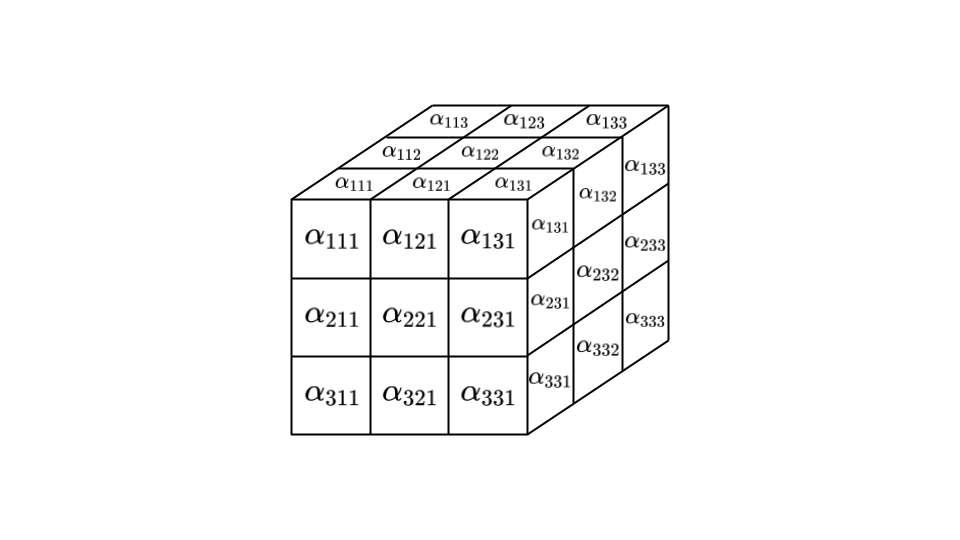
\includegraphics[width=\linewidth]{tridimensional_sup.png}
	\caption{Representación tridimensional superficial de una cubriz con elementos $\alpha_{ijk}$.}
\end{figure}

\newpage

\subsection{Tridimensional completa.}

Para una vista completa pero que conserve la estructura tridimensional, podemos separar cada ``rodaja'' de la cubriz a lo largo de un subíndice. Esta representación puede asistir en el reconocimiento de patrones.

\begin{figure}[H]
	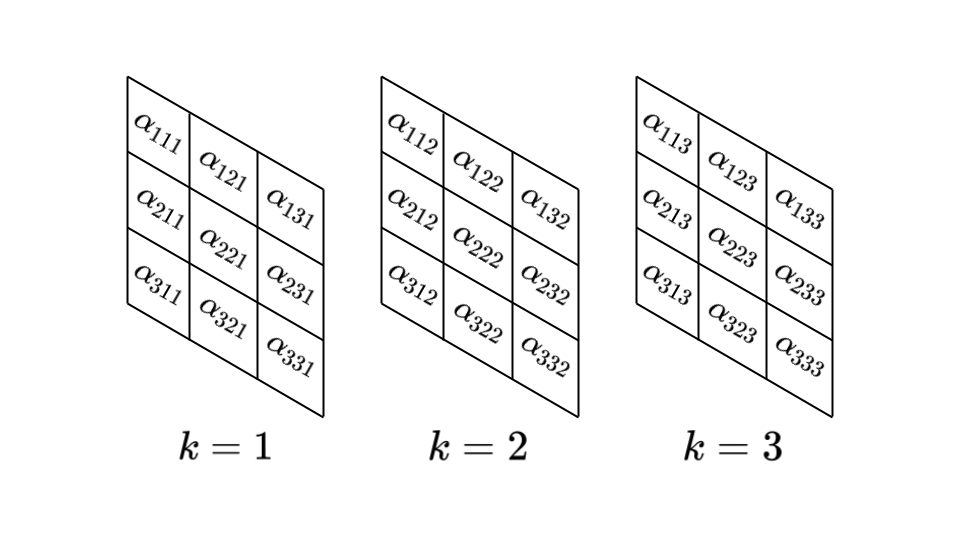
\includegraphics[width=\linewidth]{tridimensional_comp.png}
	\caption{Representación tridimensional completa de una cubriz con elementos $\alpha_{ijk}$.}
\end{figure}

\subsection{Producto.}

Bajo la definición ofrecida, el elemento $ijk$ de la cubriz $\Delta = (AB\Gamma)$ será igual al producto de la fila $i$ de $A$ por la columna $j$ de $B$ por la ``profundidad'' $k$ de $\Gamma$.

\begin{figure}[H]
	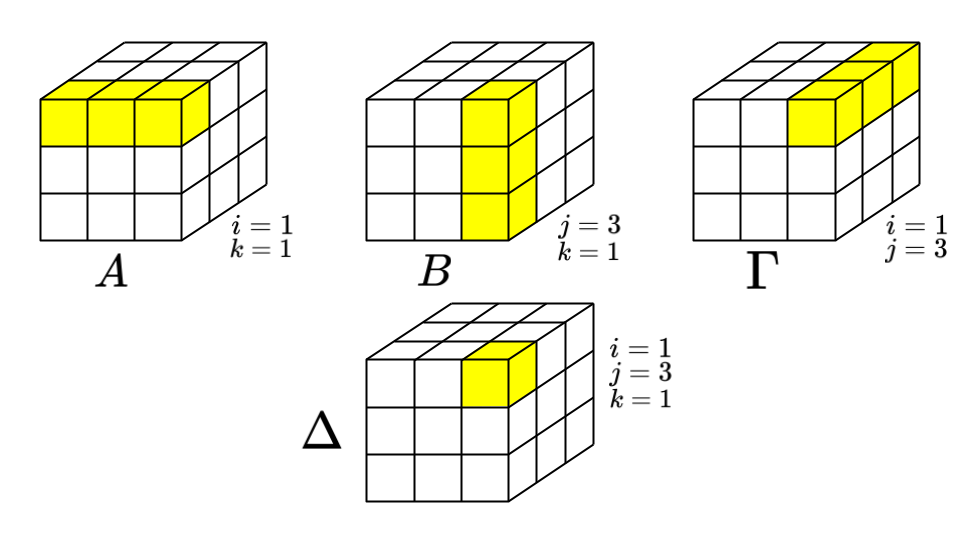
\includegraphics[width=\linewidth]{product.png}
	\caption{Representación tridimensional superficial del producto $\Delta = (AB\Gamma)$.}
\end{figure}

Esto explica las restricciones que marcan las dimensiones. En el proceso iterativo de la suma, es necesario que coincidan el número de columnas de $A$ ($n$), el número de filas de $B$ ($p$) y el número de ``profundidades'' de $\Gamma$ ($u$). Además, $\Delta$ no podrá tener más filas que $A$ ni que $\Gamma$ (de lo contrario, accederíamos a valores inexistentes), ni más columnas que $B$ o $\Gamma$, ni más ``profundidades'' que $A$ o $B$.

\section{Noción de identidad.}

La matriz identidad $I$ es aquélla que cumple que $AI = IA = A$. Es interesante buscar una noción similar en las cubrices.

\subsection{Unicidad de I.}

Sean $A, I \in M_{n} (\mathbb{K})$. Partimos de tres asunciones:

\begin{itemize}
	\item Ningún elemento de $A$ es nulo.
	\item Los elementos de $I$ no dependen de $A$.
	\item La matriz identidad $I$ es única.
\end{itemize}

Por definición:

$$A_{ijk} = (I \cdot I \cdot A)_{ijk} = \sum\limits_{l=1}^{n} I_{ilk} \cdot I_{ljk} \cdot A_{ijl}$$

y para que esto sea cierto

\begin{itemize}
	\item $I_{ilk}$ debe ser $1$ para $l = j$ y $0$ para $l \neq j$. 
	\item $I_{ljk}$ debe ser $1$ para $l = i$ y $0$ para $l \neq i$.
\end{itemize}

Pero habrá casos como $I_{122}$ donde no será posible cumplir ambas condiciones a la vez. (Véase el Anexo para un desarrollo completo en $M_2 (\mathbb{K})$ si se precisa esclarecer el patrón).

Al menos una de nuestras suposiciones debe estar errada, y sería óptimo que fuese la tercera (sobre la unicidad de la identidad).

\subsection{La identidad como par.}

Decimos que $I, J \in M_{n} (\mathbb{K})$ forman un \textit{par identidad} si cumplen que $AIJ = A$ (exploraremos más adelante la influencia del orden de los factores). Nuevamente utilizamos la definición del producto:

$$A_{ijk} = (AIJ)_{ijk} = \sum\limits_{l=1}^{n} A_{ilk} I_{ljk} J_{ijl}$$

\newpage

Esta vez las condiciones que han de satisfacerse son:

\begin{itemize}
	\item $I_{ljk} = J_{ijl}^{-1}$ para $l = j$ y $I_{ljk} J_{ijl} = 0$ para $l \neq j$.
	\item $J_{ijl} = I_{ljk}^{-1}$ para $l = k$ y $J_{ijl} I_{ljk} = 0$ para $l \neq k$.
\end{itemize}

Dos cubrices cualquiera que cumplan estas condiciones serán consideradas un \textit{par identidad}, y cumplirán que $AIJ = A$. Es evidente entonces que si $\mathbb{K}$ es un cuerpo, existirán infinitos pares identidad, mientras que si es un anillo unitario conmutativo, solo existirán los que a continuación presentamos.

\subsection{Las tres Kronecker.}

Por comodidad y estandarización, resulta inmediata la idea de establecer que todos los términos que deban ser el inverso de otros términos sean iguales a $1$, mientras que todos los que deban anularse con otro sean iguales a $0$.

Es decir, que para que $(AIJ)_{ijk} = A_{ijk}$, debe cumplirse que $I_{ljk} = J_{ijl} = \delta_{jl}$, donde

\begin{equation}
	\delta_{ab} =
	\begin{cases}
		1 & \text{si } a = b \\
		0 & \text{si } a \neq b
	\end{cases}
\end{equation}

Es posible independizar estas expresiones del subíndice $l$ al notar que en $I_{ljk}$, que $l$ sea igual a $j$ es equivalente a que $i = j$ (al ser los subíndices mudos), produciendo la expresión:

$$I_{ijk} = \delta_{ij}$$

Teniendo en cuenta que el par identidad no es conmutativo, es sencillo hacer un desarrollo similar tanto para $I_2 A J_2$ como para $I_3 J_3 A$ (conmutar la posición de $I$ y $J$ no produce nuevas cubrices, solo conmuta sus nombres), de lo cual obtendremos que:

\begin{itemize}
	\item $A I_1 J_1 = A \Leftrightarrow I_1 = \delta_{ij}$ y $J_1 = \delta_{jk}$.
	\item $I_2 A J_2 = A \Leftrightarrow I_2 = \delta_{ij}$ y $J_2 = \delta_{ik}$.
	\item $I_3 J_3 A = A \Leftrightarrow I_3 = \delta_{jk}$ y $J_3 = \delta_{ik}$.
\end{itemize}

Con esto concluímos que existen tres pares identidad estándar fundamentados sobre las tres Kronecker. No es inmediatamente obvio qué patrón se puede esclarecer de este resultado. Una posibilidad es la siguiente:

\begin{itemize}
	\item Si $I$ es adyacente a $A$, $I = \delta_{ij}$. Si no, $I = \delta_{jk}$.
	\item Si $J$ es adyacente a $A$, $J = \delta_{ik}$. Si no, $J = \delta_{jk}$.
\end{itemize}

\newpage

Sea como fuere, es intrigante observar los patrones dibujados por cada Kronecker. Tomemos sus representaciones tridimensionales completas.

\begin{figure}[H]
	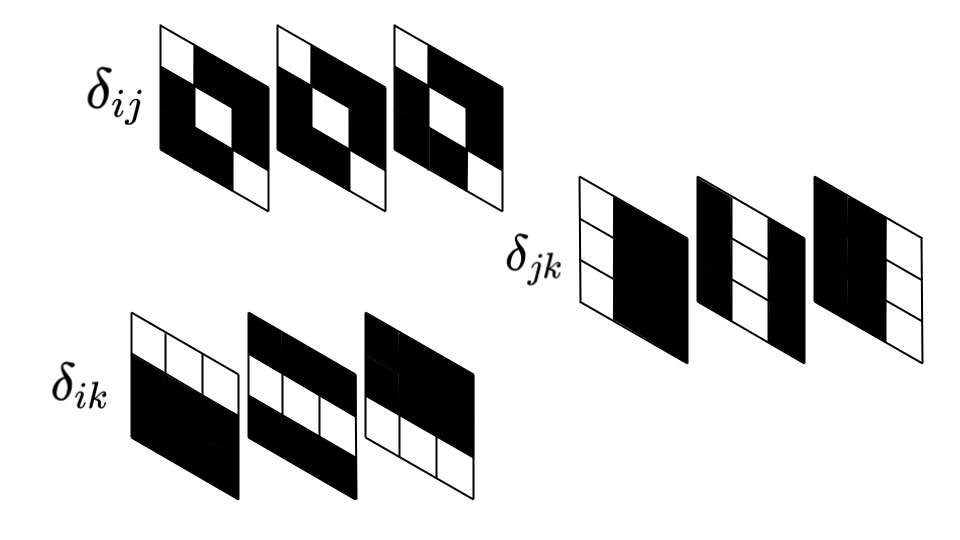
\includegraphics[width=\linewidth]{kroneckers.png}
	\caption{Representación tridimensional completa de $\delta_{ij}$, $\delta{jk}$ y $\delta{ik}$ (celdas iguales a $1$ en blanco e iguales a $0$ en negro).}
\end{figure}

\section{Noción de inversa.}

\subsection{Par inversa.}

Al igual que antes, buscamos inspiración en el área de las matrices, donde la matriz inversa $A^{-1}$ a otra matriz $A$ es aquélla que satisface que ${A\cdot A^{-1} = A^{-1} \cdot A = I}$. Ya ha quedado en evidencia la multiplicidad de las cubrices identidad, así que hemos de esperar lo mismo para las cubrices inversas.

Decimos que $(A_{ij1}^{-1})$ y $(A_{ij2}^{-1})$ forman un \textit{par inversa} sobre $i,j$ si ${A\cdot (A_{ij1}^{-1}) \cdot (A_{ij2}^{-1}) = \delta_{ij}}$. (En este caso, $(A_{ij1}^{-1})$ debe pensarse como una sola expresión o nombre. Sus subíndices son parte del nombre, por lo que algo como ``$(A_{111}^{-1})$'' carecería de sentido en este contexto).

Por definición del producto:

$$\delta_{ij} = \sum\limits_{l=1}^{n} A_{ilk} \cdot (A_{ij1}^{-1})_{ljk} \cdot (A_{ij2}^{-1})ijl$$

Si $i = j$:

$$1 = \sum\limits_{l=1}^{n} A_{ilk} \cdot (A_{ij1}^{-1})_{ljk} \cdot (A_{ij2}^{-1})_{ijl}$$

Mientras que si $i \neq j$:

$$0 = \sum\limits_{l=1}^{n} A_{ilk} \cdot (A_{ij1}^{-1})_{ljk} \cdot (A_{ij2}^{-1})_{ijl}$$

Manteniendo nuestra suposición de que ningún elemento de $A$ tiene por qué ser cero, obtenemos lo siguiente:

$$A_{ilk} \cdot (A_{ij1}^{-1})_{ljk} = 1 \Rightarrow (A_{ij1}^{-1})_{ljk} = (A_{ilk})^{-1}$$
$$(A_{ij1}^{-1})_{ljk} \cdot (A_{ij2}^{-1})_{ijl} = 0$$

Nuevamente nos enfrentamos a infinitas soluciones, pero la que aporta una interpretación más rica es la que establece que si ${i \neq j}$, entonces ${(A_{ij1}^{-1})_{ijk} = (A_{ij2}^{-1})_{ijk} = 0}$. Esta decisión nos permite arrivar a las siguientes dos conclusiones:

$$(A_{ij1}^{-1})_{ijk} = \delta_{ij} \cdot (A_{ijk})^{-1}$$
$$(A_{ij2}^{-1})_{ijk} = \delta_{ij}$$

(Nótese que el subíndice $l$ es mudo y puede ser sustituído por el equivalente posicional).

\subsection{Generalización del par inversa.}

Hemos tratado con el par inversa sobre $i, j$ y un orden de los factores concretos, pero haciendo un desarrollo similar sobre el resto de órdenes descubrimos que:

\begin{itemize}
	\item $A(A_{ij}^{-1})\delta_{ij} = (A_{ij}^{-1})A\delta_{ij} = \delta_{ij}$.
	\item $\delta_{ik}A(A_{ik}^{-1}) = \delta_{ik}(A_{ik}^{-1})A = \delta_{ik}$.
	\item $A\delta_{jk}(A_{jk}^{-1}) = (A_{jk}^{-1})\delta_{jk}A = \delta_{jk}$.
\end{itemize}

Parece ser que es posible conmutar $A$ con $(A_{ab}^{-1})$ sin alterar el resultado, y que la posición del delta de Kronecker en la expresión determina bajo qué subíndices funcionará como par inversa.

Nótese que aunque el par $(A, A^{-1})$ parezca comportarse como un par identidad, esto no es cierto cuando se opera con otras cubrices.

\section{Conclusión}

Tras este análisis descubrimos que las cubrices conforman un conjunto verdaderamente interesante a la par que misterioso. Contrario a lo que se podría presuponer, este álgebra no es retrocompatible con el de las matrices bidimensionales, si bien es cierto que los conjuntos subyacentes sí lo son.

Hemos excluido de este artículo numerosos asuntos de vital importancia que podrían ser de interés para futuras investigaciones. Nociones como el ``determinante'', el ``rango'', o una definición de igualdad entre cubrices que hiciese quizás viable su retrocompatibilidad con las matrices.

Esperamos que el presente documento sirva como incentivo para implantar la curiosidad por este álgebra en la mente del lector.

\newpage
\appendix

\section{Apéndice}

\subsection{Desarrollo completo del producto por una hipotética cubriz identidad única en $M_2 (\mathbb{K})$.}

La expresión $A = IIA$ puede ser desarrollada por la definición del producto cubricial:

\begin{equation}
A_{111} = I_{111} I_{111} A_{111} + I_{121} I_{211} A_{112}
\end{equation}

\begin{equation}
A_{112} = I_{112} I_{112} A_{111} + I_{122} I_{212} A_{112}
\end{equation}

\begin{equation}
A_{121} = I_{111} I_{121} A_{121} + I_{121} I_{221} A_{122}
\end{equation}

\begin{equation}
A_{122} = I_{112} I_{122} A_{121} + I_{122} I_{222} A_{122}
\end{equation}

\begin{equation}
A_{211} = I_{211} I_{111} A_{211} + I_{221} I_{211} A_{212}
\end{equation}

\begin{equation}
A_{212} = I_{212} I_{112} A_{211} + I_{222} I_{212} A_{212}
\end{equation}

\begin{equation}
A_{221} = I_{211} I_{121} A_{221} + I_{221} I_{221} A_{222}
\end{equation}

\begin{equation}
A_{222} = I_{212} I_{122} A_{221} + I_{222} I_{222} A_{222}
\end{equation}

En base a ese sistema derivamos lo siguiente:

\begin{enumerate}[(a)]
	\item Por $(1) \Rightarrow I_{111} = 1$.
	\item Por $(8) \Rightarrow I_{222} = 1$.
	\item Por $(3)$ y $(a) \Rightarrow I_{121} = 1$.
	\item Por $(3)$ y $(c) \Rightarrow I_{221} = 0$.
	\item Por $(6)$ y $(b) \Rightarrow I_{212} = 1$.
	\item Por $(2)$ y $(e) \Rightarrow I_{122} = 1$.
\end{enumerate}

Por $(8)$, o $I_{212}$ o $I_{122}$ deben ser $0$, pero por $(e)$ y $(f)$, $I_{212} = I_{122} = 1 \neq 0$. Surge la misma contradicción al probar con $IAI$ y $AII$.

\subsection{Desarrollo completo del producto por un par identidad en $M_2 (\mathbb{K})$.}

\begin{equation}
A_{111} = A_{111} I_{111} J_{111} + A_{121} I_{211} J_{112}
\end{equation}

\begin{equation}
A_{112} = A_{112} I_{112} J_{111} + A_{122} I_{212} J_{112}
\end{equation}

\begin{equation}
A_{121} = A_{111} I_{121} J_{121} + A_{121} I_{221} J_{122}
\end{equation}

\begin{equation}
A_{122} = A_{112} I_{122} J_{121} + A_{122} I_{222} J_{122}
\end{equation}

\begin{equation}
A_{211} = A_{211} I_{111} J_{211} + A_{221} I_{211} J_{212}
\end{equation}

\begin{equation}
A_{212} = A_{212} I_{112} J_{211} + A_{222} I_{212} J_{212}
\end{equation}

\begin{equation}
A_{221} = A_{211} I_{121} J_{221} + A_{221} I_{221} J_{222}
\end{equation}

\begin{equation}
A_{222} = A_{212} I_{122} J_{221} + A_{222} I_{222} J_{222}
\end{equation}

De manera análoga, derivamos que:

\begin{enumerate}[(a)]
	\item Por $(1) \Rightarrow I_{111} \neq 0 \neq J_{111}$ y $I_{111} = J_{111}^{-1}$.
	\item Por $(8) \Rightarrow I_{222} \neq 0 \neq J_{222}$ y $I_{222} = J_{222}^{-1}$.
	\item Por $(2)$ y $(a) \Rightarrow I_{112} = J_{111}^{-1} = I_{111} \neq 0$.
	\item Por $(6)$ y $(c) \Rightarrow I_{112} = J_{211}^{-1} \neq 0 \Rightarrow J_{211} \neq 0$.
	\item Por $(5)$ y $(d) \Rightarrow J_{211} = I_{111}^{-1} = J_{111}$.
	\item Por $(7)$ y $(b) \Rightarrow I_{221} = J_{222}^{-1} \neq 0$.
	\item Por $(3)$, $(4)$ y $(f) \Rightarrow J_{122} = I_{221}^{-1} = I_{222}^{-1} = J_{222}^{-1}$.
	\item Por $(g)$ y $(b) \Rightarrow I_{222} = J_{222}^{-1} = I_{222}^{-1} \Rightarrow I_{222}^2 = 1 \Rightarrow I_{222} = 1 = J_{222}$.
\end{enumerate}

\newpage

Recapitulando:

\begin{itemize}
	\item $I_{221} = J_{122} = I_{222} = J_{222} = 1$.
	\item $J_{211}^{-1} = I_{111} = J_{111}^{-1} = I_{112}$.
	\item El resto de términos:

	\begin{itemize}
		\item $I_{211} J_{112} = 0$.
		\item $I_{212} J_{112} = 0$.
		\item $I_{121} J_{121} = 0$.
		\item $I_{122} J_{121} = 0$.
		\item $I_{211} J_{212} = 0$.
		\item $I_{212} J_{212} = 0$.
		\item $I_{121} J_{221} = 0$.
		\item $I_{122} J_{221} = 0$.
	\end{itemize}
\end{itemize}

\begin{itemize}
	\item $1 = I_{221} = J_{122} = I_{222} = J_{222} = J_{211}^{-1} = I_{111} = J_{111}^{-1} = I_{112}$.
	\item $0 = I_{211} = J_{112} = I_{212} = J_{112} = I_{121} = J_{121} = I_{122} = J_{121} = I_{211} = J_{212} = I_{212} = J_{212} = I_{121} = J_{221} = I_{122} = J_{221}$.
\end{itemize}

Vemos que siempre se cumple que:

\begin{itemize}
	\item Si $j = 1 \rightarrow I_{1jk} = J_{ij1} = 1$ y $I_{2jk} = J_{ij2} = 0$.
	\item Si $j = 2 \rightarrow I_{1jk} = J_{ij1} = 0$ y $I_{2jk} = J_{ij2} = 1$.
\end{itemize}

El patrón se vuelve trivial si vemos qué ocurre con una cubriz $3 \times 3 \times 3$:

$$(AIJ)_{ijk} = A_{i1k} I_{1jk} J_{ij1} + A_{i2k} I_{2jk} J_{ij2} + A_{i3k} I_{3jk} J_{ij3}$$

\begin{itemize}
	\item Si $j = 1 \rightarrow I_{1jk} = J_{ij1} = 1$ y $I_{2jk} = J_{ij2} = 0$ y $I_{3jk} = J_{ij3} = 0$.
	\item Si $j = 2 \rightarrow I_{1jk} = J_{ij1} = 0$ y $I_{2jk} = J_{ij2} = 1$ y $I_{3jk} = J_{ij3} = 0$.
	\item Si $j = 3 \rightarrow I_{1jk} = J_{ij1} = 0$ y $I_{2jk} = J_{ij2} = 0$ y $I_{3jk} = J_{ij3} = 1$.
\end{itemize}

Es decir, para que $(AIJ)_{ijk} = A_{ijk}$, debe cumplirse que $I_{ljk} = J_{ijl} = \delta_{jl}$.

Como descubrimos en la sección 4.2, gracias a que los subíndices son mudos podemos llegar a las tres Kronecker.

\end{document}
